
\begin{exercise}

% !TEX root = ../main.tex



 \begin{minipage}[t]{.67\linewidth}
Een munt met een massa van \SI{3,0}{g} ligt op een blokje van \SI{20,0}{g}. Het geheel ligt op een draaiende schijf op \SI{12,0}{cm} van de rotatieas. Als de wrijvingsco\"effici\"ent tussen de munt en het blokje 0,52 is, en de wrij\-vings\-co\"effici\"ent tussen het blokje en de schijf 0,75 is, welke hoeksnelheid mag de schijf dan maximaal hebben zodat noch de munt noch het blokje wegschuift?
\end{minipage}
\hfill
\begin{minipage}[t]{.3\linewidth}
	\raisebox{1ex-\height}{%
    	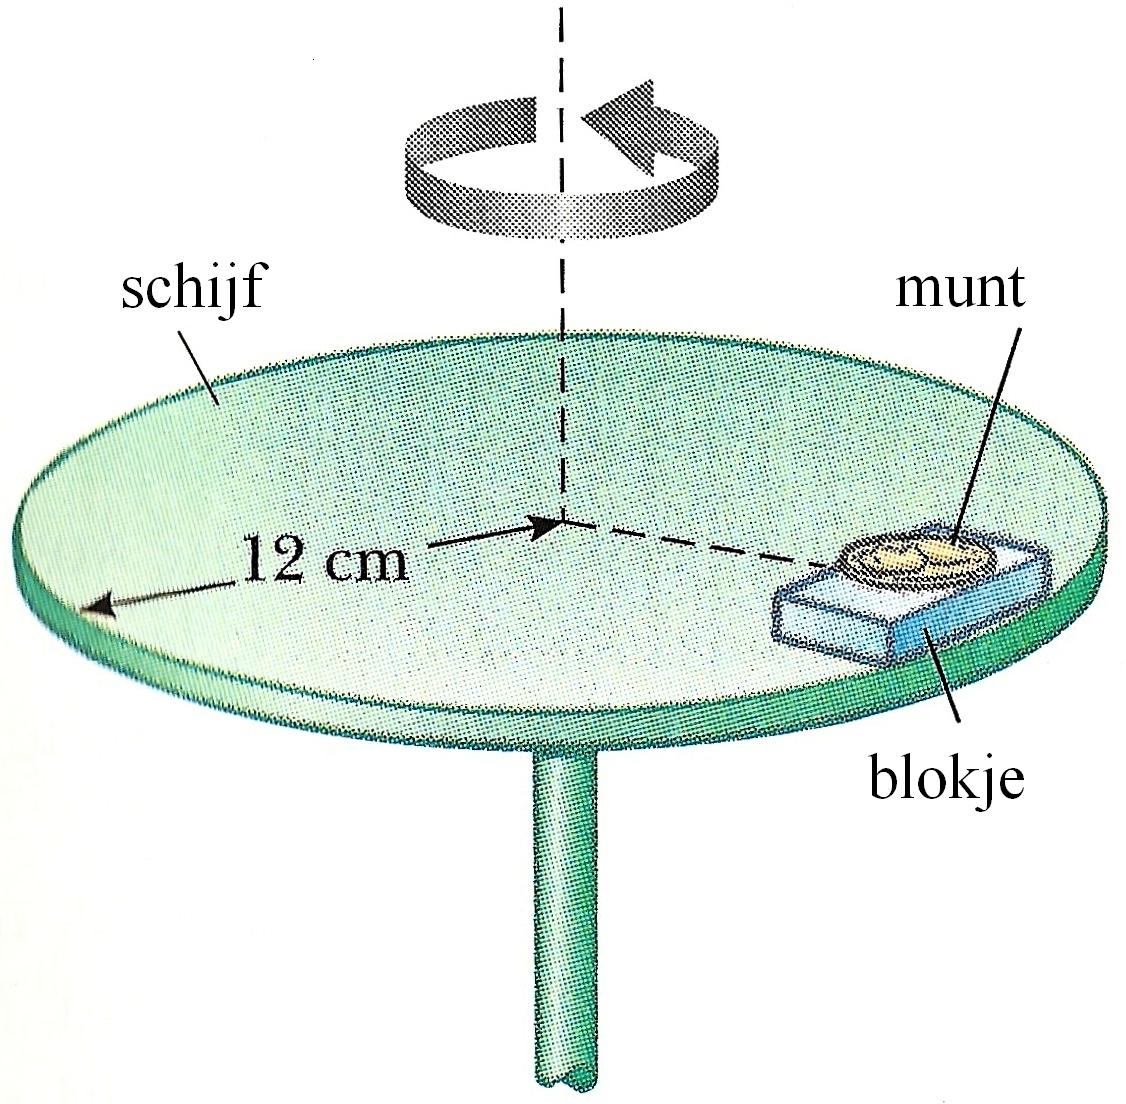
\includegraphics[width=\linewidth]{dyn/exercises/muntblokjeopschijf}%
  	}%
\end{minipage}

\begin{oplossing}
	De middelpuntzoekende kracht die nodig is om de objecten te laten ronddraaien, wordt door de wrijvingskracht geleverd. De maximale grootte hiervan wordt gegeven door $\mu F_n$. De hoeksnelheid die we nog net kunnen aanhouden zonder dat de massa's schuiven, vinden we met de tweede wet van Newton, $\vec{F}=m\vec{a}$:
	\begin{eqnarray*}
%		\vec{F}&=&m\vec{a}\\
%		&\Downarrow&\\
		\mu mg&=&mr\omega^2
		%\Leftrightarrow\omega&=&\sqrt{\frac{\mu g}{r}}
	\end{eqnarray*}
	of
		\begin{eqnarray*}
\omega=\sqrt{\frac{\mu g}{r}}
	\end{eqnarray*}
	
Hierin hebben we gebruikt dat de massa's in de verticale richting niet versnellen en dus de normaalkracht op de massa's even groot is als de zwaartekracht op die massa's. Ook hebben we gebruikt dat de versnelling van een object dat een eenparig cirkelvormige beweging uitvoert, gegeven wordt door $a=r\omega^2$.

Omdat de massa geen rol\footnote{De massa speelt geen rol omdat hij niet in de formule voorkomt. Dat is een hard wiskundig argument. Een kwalitatieve uitleg is dat voor een grotere massa weliswaar een grotere middelpuntzoekende kracht nodig is maar dat de normaalkracht ook evenredig groter wordt met de massa, en dus ook de wrijvingskracht.} speelt in deze formule, bepaalt de kleinste $\mu$ de maximale hoeksnelheid:
 \begin{eqnarray*}
\omega=\sqrt{\frac{\mu g}{r}}=\SI{6,52}{rad/s}
	\end{eqnarray*}
\end{oplossing}

\end{exercise}
